\section{Transcrição}
\frame{ \justifying
     \frametitle{Início da regulação de um gene}
     \begin{itemize}
		\item Um dos primeiros passos para a expressão de um gene é a transcrição.
		\item Onde diversos fatores podem influenciar a indução ou a repressão da expressão.		     
     \end{itemize}
%O primeiro passo na expressão de um gene é a transcrição. No processo de transcrição muitos fatores internos ou externos, na célula, podem influenciar induzindo ou reprimindo a expressão dos diversos genes codificados no genoma do organismo. Fatores externos desafiantes, como estresses bióticos e abióticos, até mecanismos moleculares intrínsecos podem desencadear, direta ou indiretamente, a ativação da expressão gênica espaço-temporal.
}

\frame{ \justifying
	\frametitle{Ácidos nucleicos}
	\begin{itemize}
		\item Os ácidos nucleicos são importantes moléculas que contem o material genético da célula.
		\item Uma analogia de sistemas biológicos com sistemas de computadores é pensar nos ácidos nucleicos como um código objeto de um programa, onde este código é descifrado pelo o sistema operacional (a célula) que irá tomar as devidas ações. No caso de células a ação é a produção de proteínas.
	\end{itemize}
% Na transcrição de um gene há diversos atores que trabalham em conjunto mas cada um com tarefaz específicas, uns desses autores são os ácidos nucleicos.
}

\frame{ \justifying
	\frametitle{Ácidos nucleicos}
	\begin{itemize}
		\item A composição química dos ácidos nucleicos é: um açúcar, uma base nitrogenada e um ácido fosfórico.
		\item Eles são ligados formando uma sequência linear.
	\end{itemize}
}

\frame{ \justifying
	\frametitle{Ácidos nucleicos}
\begin{figure}[htb!]
    \centering
    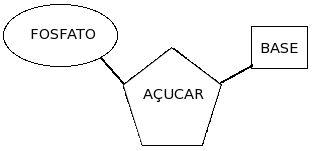
\includegraphics[scale=0.7]{./imagens/componentes_nucleotideo.png}
    \caption{Componentes de um nucleotídeo}
    \label{fig:nucleotideo}
\end{figure}
}

\frame{ \justifying
	\frametitle{Ácidos nucleicos}
\begin{figure}[htb!]
    \centering
    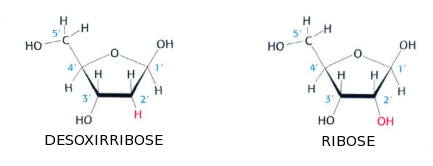
\includegraphics[scale=0.7]{./imagens/tipos_acucar.png}
    \caption{Tipos de açúcar encontrados nos ácidos nucleicos. \cite[Adaptada]{Berg2007})}
    \label{fig:tipos_acucar}
\end{figure}
}

\frame{ \justifying
	\frametitle{Ácidos nucleicos}
\begin{figure}[htb!]
    \centering
    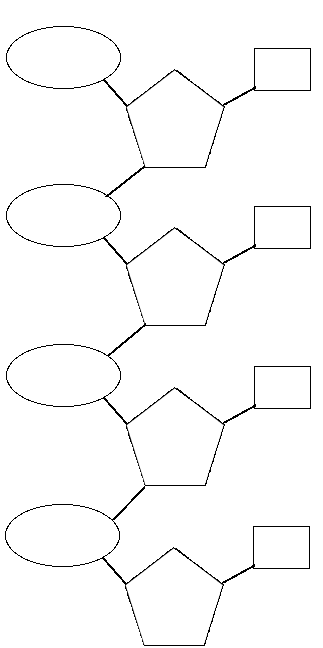
\includegraphics[scale=0.3]{./imagens/sequencia_nucleotideo.png}
    \caption{Sequência linear de nucleotídeos ligados}
    \label{fig:sequencia_nucleotideo}
\end{figure}
}


\frame{ \justifying
	\frametitle{Ácidos nucleicos}
	Existem dois tipos de ácidos nucleicos:
	\begin{enumerate}
		\item Ácido desoxirribonucleico (DNA)
		    \begin{itemize}
		    	\item açúcar: desoxirribose
		    	\item bases: A,\textbf{T}, G e C
		    	\item estrutura: duas sequências complementares pareadas formando um helicoide
		    \end{itemize}
		\item Ácido ribonucleico (RNA)		
		    \begin{itemize}
		    	\item açúcar: ribose
		    	\item bases: A, \textbf{U}, G e C
		    	\item estrutura: única sequência de nucleotídeos
		    \end{itemize}
	\end{enumerate}
	
}
	
\frame{ \justifying
	\frametitle{Ácidos nucleicos}
\begin{figure}[htb!]
    \centering
    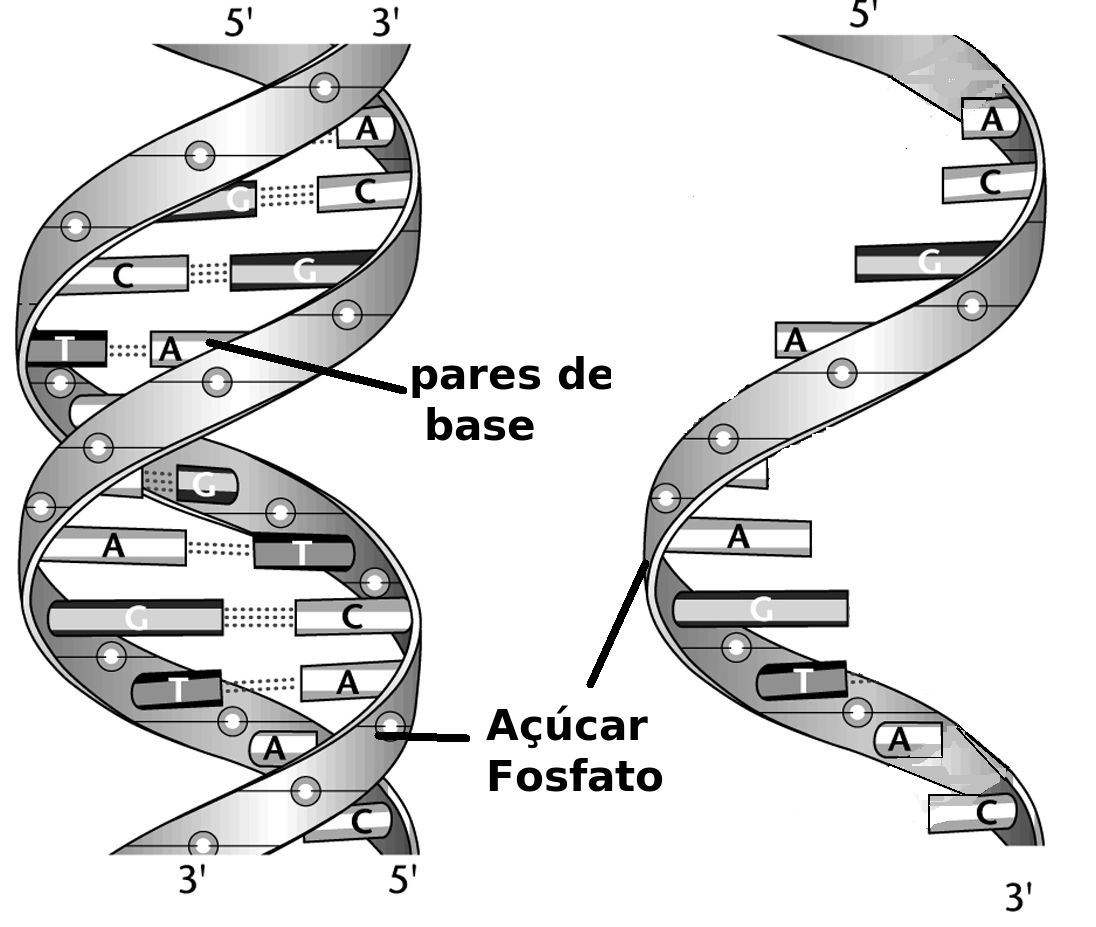
\includegraphics[scale=0.7]{./imagens/estrutura_DNA_RNA.jpg}
    \caption{Estrutura do DNA e RNA. \cite[Adaptada]{Higgs2005}}
    \label{fig:estrutura_DNA_RNA}
\end{figure}
}

\frame{ \justifying
	\frametitle{Transcrição}
	\begin{itemize}
		\item A transcrição consiste na formação do RNA a partir do DNA.
		\item É feita uma cópia exata de um segmento de DNA.
		\item Parte do RNA formado será usado na síntese de proteínas.
%		\item Os genes contém as informações que especificam um tipo de proteína.
		\item Todo esse processo é conhecido como dogma central.
	\end{itemize}
}

\frame{ \justifying
	\frametitle{Transcrição}
\begin{figure}[htb!]
    \centering
    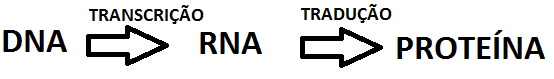
\includegraphics[scale=0.7]{./imagens/passo_expresscao_genica.png}
    \caption{Principais passos da expressão de genética}
    \label{fig:passo_expresscao_genica}
\end{figure}
}

\frame{ \justifying
	\frametitle{Transcrição}
		\begin{itemize}
			\item Para que ocorra a transcrição é necessário a ação de uma enzima chamada RNA-polimerase.
			\item Ela se conecta no DNA juntamente com fatores de transcrição gerais (formando um complexo)
			\item A RNA-polimerase se movimenta na direção 5' $\rightarrow$ 3' formando o RNA.
		\end{itemize}
}

\frame{
	\frametitle{Transcrição}
		\begin{figure}[htb!]
		    \centering
		    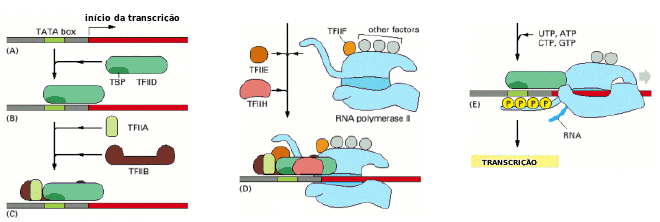
\includegraphics[scale=0.65]{./imagens/complexo_RNA-polimerase.png}
		    \caption{RNA polimerase e os fatores de transcrição gerais \cite[Adaptada]{Alberts2002} }
		    \label{fig:complexo_RNA-polimerase}
		\end{figure}
}

\frame{ \justifying
	\frametitle{Transcrição}
\begin{figure}[htb!]
    \centering
    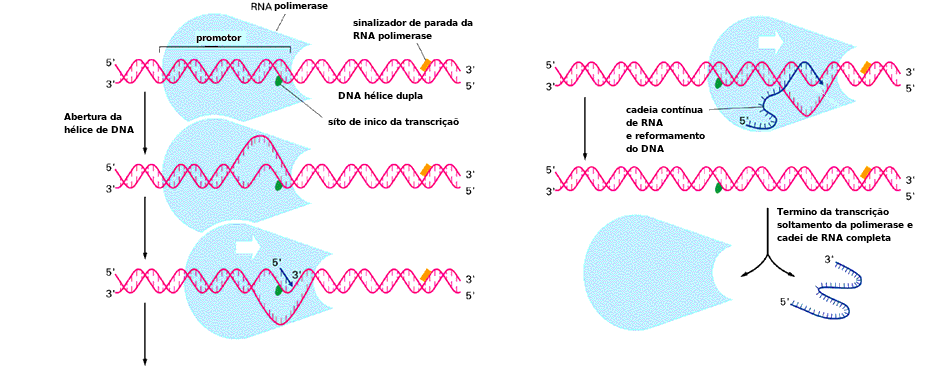
\includegraphics[scale=0.45]{./imagens/RNAPOLII.png}
    \caption{Formação do RNA através da RNA polimerase \cite[Adaptada]{Higgs2005}}
    \label{fig:RNAPOLII}
\end{figure}
}